\chapter{Implementierung und Benchmarks}
Es wurde der in Kapitel 3 beschriebe Algorithmus zur Berechnung der QR-Zerlegung mittels Householder-Transformation implementiert. Außerdem wurde sich an der Implementierung von LAPACK orientiert.

Es wurde der Ungeblockte und der Geblocket Algorithmus implementiert. Beide Algorithmen wurden mit BLAS routinen der IntelMKL implementiert. Die Implementiertung wurde dann mit den Algorithmen der IntelMKL verglichen.

Die Implementierung steht auf GitHub Verfügung \cite{git}.\\
\url{https://github.com/Flousen/Bachelorarbeit}

\section{Bibliothek}
Die verwendete Bibliothek wurde in der Vorlesung High Performance Computing 1 entwickelt \cite{HPC1}.

Die Bibliothek ist in C++ geschrieben. Es sind Klassen für Matrizen und Vektoren implementiert, sowie einige BLAS-Routinen.

Die Matrix-Klassen erlauben den zugriff auf Matrixblöcke. 
Der folgender Code Soll Beispielhaft den Zugriff auf Matrixblöcke veranschaulichen.
\begin{lstlisting}
GenerelMatrix<T> A(5,5);  // erzeuer Matrix Objekt
init(A);  // Matrix mit zufalls Zahlen initialisieren
printf("A   =\n");print(A); // Matrix Ausgeben
printf("A22 =\n");print(A.block(2,2));
printf("A22T=\n");print(A.block(2,2).view(Trans::view));
\end{lstlisting}

Dieser Code kann die folgende Ausgabe erzeugen. \newpage
\lstset{numbers=none}
\begin{lstlisting} 
A   = 
      1    2    3    4    5
      6    7    8    9   10
     11   12   13   14   15
     16   17   18   19   20
     21   22   23   24   25

A22 = 
     13   14   15
     18   19   20
     23   24   25

A22T= 
     13   18   23
     14   19   24
     15   20   25
\end{lstlisting}

\subsubsection{MKL Wrapper}
\lstset{numbers=left,firstnumber=14}
\begin{lstlisting}
double
dot(MKL_INT n, const double *x, MKL_INT incx,
    const double *y, MKL_INT incy)
{
  return ddot(&n, x, &incx, y, &incy);
}

template <typename T, template<typename> class VectorX,
                      template<typename> class VectorY,
          Require< Dense<VectorX<T>>,
                   Dense<VectorY<T>> > = true>
T
dot(const VectorX<T> &x, const VectorY<T> &y)
{
  return dot(x.length(), x.data(), x.inc(), 
             y.data(), y.inc());
}
\end{lstlisting}


  

\subsection{Algorithmus}

Beispiel Ungeblockte QR Implementierung vom Algorithmus \ref{alg:unblockedqr}
\lstset{numbers=left,firstnumber=1}
\begin{lstlisting}
size_t mn = std::min(m,n);
DenseVector<T> work(mn);
for (std::size_t i = 0; i < mn; ++i){
  householderVector(A(i,i), A.col(i+1,i),tau(i));
  if (i < n && tau(i) != 0) {
    AII = A(i,i);
    A(i,i) = 1;
    mv(1, A.block(i,i+1).view(hpc::matvec::Trans::view),
       A.col(i,i), 0, work.block(i+1));
    rank1(-tau(i), A.col(i,i), work.block(i+1), 
          A.block(i,i+1));
    A(i,i) = AII;
  }
}
\end{lstlisting}

Die anderen Algorithem wurden analog Implementiert siehe Anhang.

\section{Fehlerschätzer}

Um zu testen ob die QR-Zerlegung korrekt ist, ist ein Fehlerschätzer notwendig.
Es wurde der Fehlerschätzer von ATLAS \cite{atlas} verwendet.
\begin{align}
err = \dfrac{\|A - QR\|_i}{\|A\|_i \cdot \min(m,n) \cdot \varepsilon}
\end{align}
$\|\cdot\|_i$ ist eine passende Norm.
Die Matrizen $Q$ und $R$ sind die QR-Zerlegung der Matrix $A \in \mathbb{R}^{m \times n}$.
$\varepsilon$ ist die kleinste darstellbare Zahl.\\
Die QR-Zerlegung ist gut genug falls der Fehler kleiner 1 ist: $ err < 1 $.

Als Norm wurde die Zeilensummennorm $\|\cdot\|_\infty$ gewählt.
Diese ist für eine Matrix $A \in \mathbb{R}^{m\times n}$ gegeben durch
\begin{align*}
\|A\|_\infty = \max_{i=1,...,m} \sum_{j=1}^{n} |a_{ij}|
\end{align*}

Diese Norm wurde gewählt, da sie für zeilenweise gespeicherte Matrizen effizient berechnet werden kann.

\section{Benchmarks}

\subsection{Aufwand}

Der Aufwand der QR-Zerlegung mittels Householdertransformation einer Matrix $A \in \mathbb{R}^{m \times n}$  \cite{atlas} angegeben mit.
\begin{align*}
%\# &= n^2(m-\frac{1}{3} n) + {\cal O}(mn) \\
\# &= n \cdot \left(\frac{23}{6} + m + \dfrac{n}{2} + n\cdot \left(\frac{m-n}{3} \right) + n\cdot \left(\dfrac{5}{6} + \dfrac{n}{2} + m - \dfrac{n}{3}\right)\right)
\end{align*}
$\#$ bezeichnet die Anzahl der Rechenoperationen. 

\subsection{FLOPS}
FLPOS (Floating Point Operations Per Second) geben an wie viele Fließkomma Operationen pro Sekunde ausgeführt werden.

\begin{align*}
  \text{FLPOS} = \dfrac{\#}{\Delta t}
\end{align*}

$\Delta t$ bezeichnet die Zeit in Sekunden und $\#$ die Anzahl der Rechenoperationen, die zur Berechnung der QR-Zerlegung, einer $m \times n$ Matrix, benötigt wird.



\subsection{Test System}

Getestet wurde auf einem System mit einer Intel(R) Core(TM) i5-3470 CPU mit 3.20GHz. 

Die Theoretische peak performance errechnet sich aus der Taktrate mal die Registerbreite mal 2. 



Die CPU des Test Systems hat eine Taktrate von 3.20GHz.
Die AVX-Register sind 256-Bit groß. Darin haben 4 double Platz.

\begin{align*}
  \text{Taktrate} \cdot \text{Registerbreite} \cdot 2= 3,20 \text{ GHz} \cdot 4 \cdot 2 = 25,6 \text{ GFLOPs}
\end{align*}

\begin{figure}[H]
  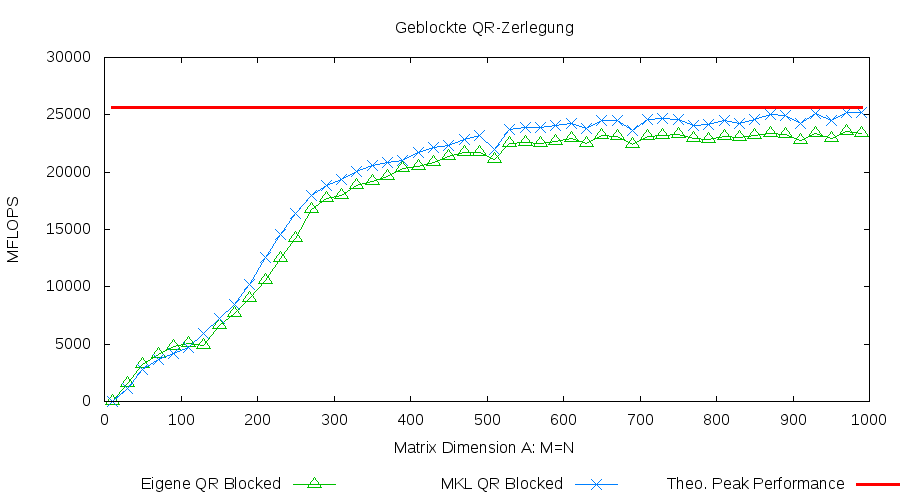
\includegraphics[width=\textwidth]{images/blk.png}
  \caption{Benchmark geblockte QR-Zerlegung}
  \label{img:blk}
\end{figure}

\begin{figure}[H]
  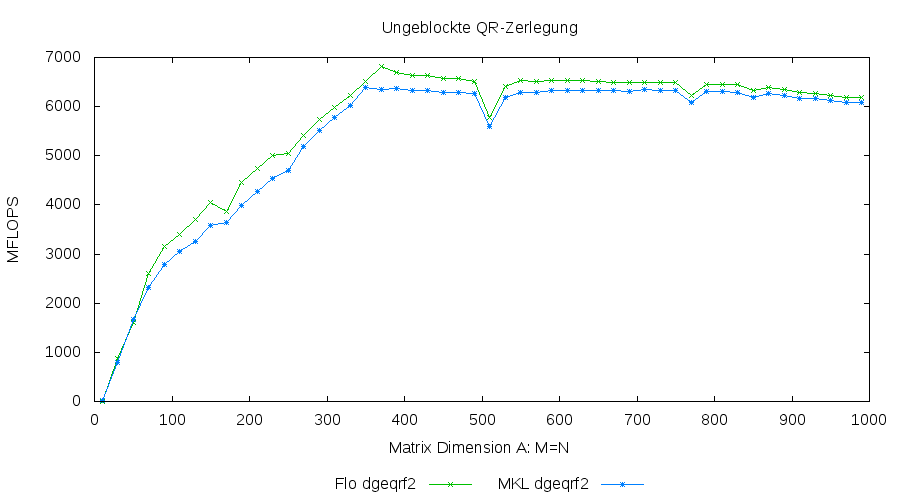
\includegraphics[width=\textwidth]{images/unblk.png}
  \caption{Benchmark ungeblockte QR-Zerlegung}
  \label{img:unblk}
\end{figure}








   
